\chapter{Methodology}

As there are no publically available datasets with images of pain assessment in fetus, our work was developed in conjunction with the group of studies of Fetal Pain Assessment from the Univeristy of São Paulo (USP), which studies pain assessment in fetuses and was responsible for collecting the images.

Videos were recorded in three groups. The first one for control purposes, was just with fetuses in resting conditions. The second one was of fetueses that had to go trough an intra-uterin surgery, and thus needed fetal anesthesia, in this case the exact moment when the needle was applied was recorded. This recorded the reaction of the fetus in pain, and in some cases even crying. Notice that these videos also had images (1) a baseline period defined as the least 30 seconds before the anaesthesia puncture and (2) the 45 seconds immediately after the puncture. Finally the third group of videos was recorded while the fetus was exposed to the sound of horn, this was meant to cause distress but it should be a control group rather different from pain which we expected to differentiate.

Videos were recorded from the 4D Ultrasound machine of the model Voluson E8 by GE. 

We had a total of 15 videos to work with, with 5 from each group.

For the images collected during fetal anesthesia, a second ultrasound machine was placed in the clinical room, as the main one was used for the medical procedure of the puncture and the second one was used to target the fetus face an to monitor its expressions.

These images with fetus in pain conditions were evaluated by 3 professionals with the NFCS scale, and these evaluations could further be used to quantify the amount of pain 

\section{Image Sampling}

Notice that it is common to have an small number of data to work with as this is a very hard data to collect. Only a small percentage of the fetus have to go trough surgery prior to birth, and thus fetal anesthesia is a relatively rare procedure. Other studies also have a small N, like these ones ... 

In order to deal with the limited amount of data, we've decided to deal with this problem in another dimension. We reduced the space from videos to images. In orther to do this, we decided to sample the videos at the hate of every 2 seconds. With this processes we created a total of 268 images.

But as the images were recorder from ultrasound machines, they depend on the calibration by the doctors in orther to capture the exact section in the 3 dimensional space where the fetus face is. Because of this, it is common for this type of image to have a lot of noise, and thus some of the sampled images did not contain a clear face of the fetus. This was a problem, as we had a significant number of images, and manual selection would not only hard by non deterministic.

So in orther to overcome this issue, we decided to use a neural network capable of detecting facial landimarks, like the nose, the mouth and the eyes. The network we used was the MTCNN \cite{} which was originally developed to recognize X. But it worked surprisingly well in our domain, even though the images had a quite different characteristics.

With this process, we were able to filter out our dataset of images from 268 to 145, and were sure the images contained a clear face. The network also returned a confidence number of which it found the face in the image, and we've used only confidences of over 95\%, which on manual inspection was very reliable, with just 6 errors that were removed manually.

With the position of the facial landmakrs, another process was to crop the images around the face of the fetus. This cropping is done just by adding a padding to the places were the image was. This process is also available trough the MTCNN library, and we can also add face alignement. This way, we avoid the blurred surrounding around the fetus wich contains fragments of the womb and other non distinguishable parts. 

At this point, manual inspection was needed in other to separate the images back into the three groups. With the resting images, it was easy as all the frames were from resting positions. But with the ones from anestheasia and from the horn we had to split the data between before the stimulus and after it. This was not a though process as we knew exactly when the stimuli was applied and a clear difference in the facial expression could be noted. After this step we ended up with 117 images which had a clear face on it.

\begin{figure}[h!tp]
    \centering
    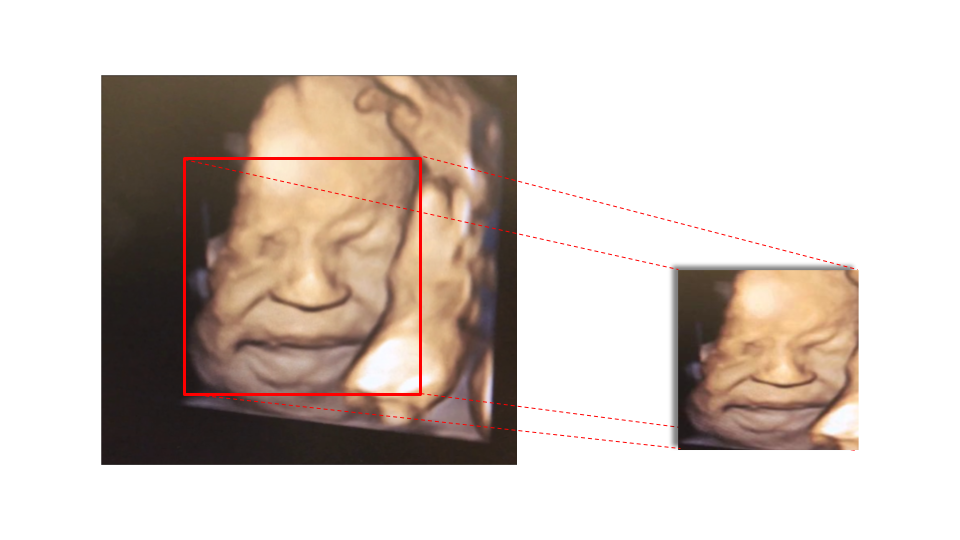
\includegraphics[width=.9\textwidth]{imgs/chap3_cropping.png}
    \caption{Image cropping with MTCNN}
    \label{fig:cropping}
\end{figure}

\section{Data Augmentation}

Even though we had increased the size of the dataset by turning the videos into images, it was still considered a small dataset for deep learning models. 

In orther to further augment our chances of succeding, we have applied the use of data augmentation techniques to increase the variability of our data. The effectiveness of such technique has been demonstrated by \cite{abs-1712-04621} and is widely used in many applications.

There is a range of possibilities for using data augmentation, the ones we've chosen are:

* Horizontal flip, which consists in mirroring the image horizontally. 
* Rotation, which consists in applying small rotations to the image
* Zoom, which consists in zooming in the image
* Ligthning, which consists in changing the britghness and the contrast of the image
* Warping, which consists in warping the image. 

All of these methods have a probability of being applied, and can be used in combination with each other. Thus for each image, given the probability, a combination of these techniques would be applied. 

\begin{figure}[h!tp]
    \centering
    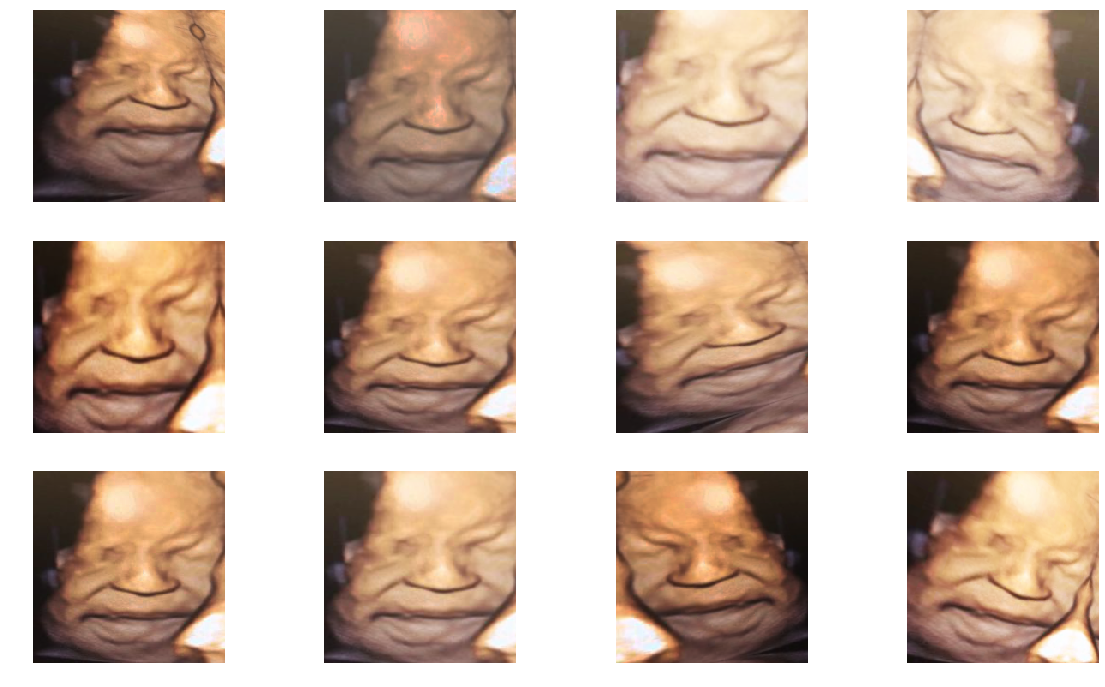
\includegraphics[width=.9\textwidth]{imgs/chap3_data_augmentation.png}
    \caption{The same image with different data augmentation applied}
    \label{fig:data_augmentation}
\end{figure}

In order to further experiment with this, we have compared 3 sets of intensity in the changes. A smooth, which does more subtle changes, a medium one, which is intensifies a little bit and a more aggressive one, wich havily transforms the images.  

\subsection{Network Architecture and Transfer Learning}

The network used was VGG with pretrained model on VGG Face



